\section{Method}

\subsection{Dataset}

Though several \gls{mri} and \gls{ct} datasets available, for instance,
\gls{oasis}~\cite{OASIS} or \gls{adni}~\cite{ADNI}, public datasets in which
both modalities are obtainable for the same subject are, to date, rare. To our
knowledge only the \gls{rire} project~\cite{RIRE} and the Cancer Imaging
Archive~\cite{CIA} provide \gls{mri} and \gls{ct} from the same subject. For
the present work we used the data from the \gls{rire} project because it uses
an uniform data fromat.
\begin{table}[h]
  \centering
  \begin{tabular}{*{6}{c}}
    \toprule
    \acrshort{ct} &
		\acrshort{mri} \acrshort{pd} &
		\acrshort{mri} \acrshort{t1} &
		\acrshort{mri} \acrshort{t2} &
		\acrshort{mri} \acrshort{mp} \acrshort{rage} &
		\acrshort{pet} \\
    \midrule
    \num{17} & \num{14} & \num{19} & \num{18} & \num{9} & \num{8} \\
             & \num{12} & \num{17} & \num{16} & \num{9} & \num{6} \\
    \bottomrule
  \end{tabular}
  \caption{Subject counts of the \gls{rire} dataset with respect to the
    available imaging modalities. In the second table row we only consider
    subjects with \gls{ct} data present.
  }\label{tab:rire}
\end{table}
In \Cref{tab:rire} we list the aggregated modality count of the \gls{rire}
dataset in the first row. In the second row we list the aggregated modality
count for the subjects with \gls{ct} modality available. Beside of \gls{ct}
one can also obtain \gls{pet} images for some subjects. Next to the common
\gls{t1} and \gls{t2} weighted \gls{mri}, some subjects of the \gls{rire}
dataset also offer \gls{pd} and \gls{mp} \gls{rage} weighted \gls{mri}s. Some
\gls{mri}s can be obtained in a rectified version, which we did not use. We
used the \gls{t1} weighted \gls{mri} together with the \gls{ct} as input and
target data as these give us the highest subject count. However, it would be
an interesting experiment to supply different \gls{mri}s as multi-channel
input. The \num{17} subjects were divided into \gls{13} subjects for training
and \gls{4} subjects for validation. We respected the transverse resolution,
i.e.\ the number of transverse slices, for the division of the dataset, in
that the validation subjects offer a high transverse resolution.

\subsection{Preprocessing}

The modality data for each subject can be downloaded from the website of the
\gls{rire} project, see Ref.~\cite{RIRE}. In \Cref{fig:conversion} we depicted
the first preprocessing protocol. It involves the extraction, decompression and
conversion of the volumetric data. After extraction and decompression the
volumetric data presents itself as \gls{mhd}. We converted the \gls{mhd} files
to the self-contained \gls{nifti} format through the Python front-end of the
\gls{itk} library.
\begin{figure}[h]
  \centering
  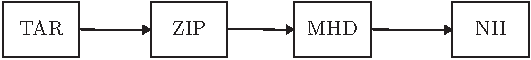
\includegraphics[page=1,width=.8\linewidth]{figure/diagrams.pdf}
  \caption{Image extraction and conversion from \gls{mhd} to \gls{nifti}
		format.
	}\label{fig:conversion}
\end{figure}
\Cref{fig:registration} illustrates the coregistration procedure that follows
the first preprocessing procedure. The coregistration yields a rigid
transformation that aligns the moving volume with the fixed volume. Given a
rigid transformation, a linear interpolator returns a translated volume from
the sample points of the initial moving volume. The mutual information between
the moved \gls{mri} and the \gls{ct} is then used to optimize the
rigid transformation. This procedure is executed iteratively and stopped when
the maximum iterations steps are reached or the convergence condition is met.
As the implementation of the interpolator and the transformation optimizer
are complex, we used the registration toolset included in the \gls{itk}
library, see Ref.~\cite{Yaniv2018}.
For the present work we choose the \gls{ct} volume to be fixed, as the
\gls{ct} volumes are in general spatially normalized accross different
subjects.
\begin{figure}[h]
  \centering
  \includegraphics[page=2,width=.8\linewidth]{figure/diagrams.pdf}
  \caption{Multi-modal image coregistration using maximum mutual information
    optimization.
	}\label{fig:registration}
\end{figure}
Following the coregistration, we used the binary fill holes algorithm from
SciPy~\cite{SciPy} to remove the \gls{ct} table present in some \gls{ct}
volumes as well as well as the background noise.\footnote{The complete
preprocessing described so far is available at
\url{https://github/bodokaiser/mrtoct-scripts}.} Finally we converted the
preprocessed pairs of \gls{mri} and \gls{ct} volumes to the tfrecord format
in order to easily read the data into Tensorflow~\cite{Tensorflow15}. As part
of the data pipeline implemented with Tensorflow we perform a pad or crop to
either $384\times384$ for transverse 2D slices. In the 3D case we perform
patch extraction of target shape $32\times32\times32$ for \gls{mri} and
$16\times16\times16$ for \gls{ct}. The target shape for the 2D slices was
choosen to be compatible with the convolution parameters and the largest
resolution of all volumes. Furtheremore we applied a min-max-normalization in
order to keep floating range arthimetic in a range of $[0,1]$.

\subsection{Models}

We implemented three different neural network models for the \gls{mri} to
\gls{ct} synthesis task. The first and most simple model is based on the
u-net model~\cite{Ronneberger15} and uses standard error metric, i.e.\
\gls{mae} and \gls{mse}. The second model is based on pix2pix~\cite{Isola16},
which already has proven great success in the task of image translation. It
uses the first u-net based model as generator in addition to a discriminator
model to calculate the adversarial loss. As third model we implemented the
context-aware 3D synthesis GAN from Nie~\cite{Nie16}. In comparison to the
other two models, which operate on the transverse 2D slices of the brain, it
is applied to 3D patches. Training an interferenc was implemented using
Tensorflow~\cite{Tensorflow15}.\footnote{The implementation is available at
\url{https://github/bodokaiser/mrtoct-tensorflow}.}

\subsubsection{u-net}

The original u-net model~\cite{Ronneberger15} was developed for the
segmentation of biomedical images. A central concept of the architecture is to
combine the capture of context and precise localization through interconnected
layers.
\begin{figure}[h]
  \centering
  \includegraphics[page=3,width=.8\linewidth]{figure/diagrams.pdf}
  \caption{The u-net architecture.
  }\label{fig:unet:gen}
\end{figure}
In \Cref{fig:unet:gen} the u-net architecture is illustrated. We remark the
two paths of data flow: for one the image is passed through a seqeunce of
encoders and decoders, then again data can flow from one encoder stage
directly to the corresponding decoder stage. The encoder encode localized
features while the decoders decode an image from the previous layer and the
corresponding encoder stage.
In comparison to the original u-net we reduced the convolution layers and
replaced the max pooling in the decoder blocks with deconvolution (also called
transposed convolution) layers. Furthermore we used Leaky ReLUs in the
encoders instead of usual ReLUs. Except for the first encoder we applied batch
normalization inbetween the convolution and activation. Another novelty
relative to the original u-net is the use of dropout layers in the first and
second decoder. Dropout layer are known to improve network generalization by
randomly suppressing features from the training process~\cite{Srivastava2014}.
The changes to the original u-net architecture are mainly inspired by the
u-net like generator used in pixtopix.
\begin{table}[h]
  \centering
  \begin{tabular}{cccc}
    \toprule
    Type & Kernel & Strides & Output Shape \\
    \midrule
    Input & & & \num{384x384x1} \\ 
    Convolution & \num{4x4} & \num{2} & \num{192x192x64} \\
    Convolution & \num{4x4} & \num{2} & \num{96x96x128} \\
    Convolution & \num{4x4} & \num{2} & \num{48x48x256} \\
    Convolution & \num{4x4} & \num{2} & \num{24x24x512} \\
    Convolution & \num{4x4} & \num{2} & \num{12x12x512} \\
    Deconvolution & \num{4x4} & \num{2} & \num{24x24x512} \\
    Deconvolution & \num{4x4} & \num{2} & \num{48x48x512} \\
    Deconvolution & \num{4x4} & \num{2} & \num{96x96x256} \\
    Deconvolution & \num{4x4} & \num{2} & \num{192x192x128} \\
    Deconvolution & \num{4x4} & \num{2} & \num{384x384x64} \\
    Deconvolution & \num{3x3} & \num{1} & \num{384x384x1} \\
    Output & & & \num{384x384x1} \\ 
    \bottomrule
  \end{tabular}
  \caption{Network parameters used in the u-net.
  }\label{tab:unet:gen}
\end{table}
\Cref{fig:unet:gen} lists the network parameters used for our u-net
architecture. The kernel paremeter specifies the shape of the convolution
kernel, the stride parameter describes the spacing between convolutions.
Weight initialization was performed using Xavier, see Ref.~\cite{Xavier2010},
if not noted otherwise.

\subsubsection{pixtopix}

The pixtopix model uses the previously introduced u-net architecture as
generator to translate an input \gls{mri} to \gls{ct}. In addition, pixtopix
utilizes a second network, the discriminator network, to output a score map
that distinguishes between real and fake \gls{ct}. In this context real
\gls{ct}s correspond to the target \gls{ct} provided by the training dataset
and fake \gls{ct}s correspond to the output \gls{ct} provided by the
generator. In this sense one is able to add an adversarial loss term to the
standard metric loss, that maximizes the identification of real \gls{ct}s
while minimizing the missidentification of fake \gls{ct}s as real
ones~\cite{Goodfellow14}.
The pixtopix model has proven great success as general purpose solution
for translation experiments with color images~\cite{Isola16}. Recently
pixtopix was extended to support even training on unpaired
data~\cite{Zhu2017}. This approach has also successfully been applied to the
task of \gls{mri} to \gls{ct} translation~\cite{Wolterink17}.
\begin{figure}[h]
  \centering
  \includegraphics[page=4,width=.8\linewidth]{figure/diagrams.pdf}
  \caption{The pixtopix discriminator architecture.
	}\label{fig:pixtopix:disc}
\end{figure}
\Cref{fig:pixtopix:disc} depicts the pixtopix discriminator architecture. It
consists of five convolution layers with non-linear activation function. The
first four activation functions are Leaky ReLUs while the last one is of type
sigmoid.
\begin{table}[h]
  \centering
  \begin{tabular}{cccc}
    \toprule
    Type & Kernel & Strides & Output Shape \\
    \midrule
    Input & & & \num{384x384x2} \\ 
    Convolution & \num{4x4} & \num{2} & \num{192x192x64} \\
    Convolution & \num{4x4} & \num{2} & \num{96x96x128} \\
    Convolution & \num{4x4} & \num{2} & \num{48x48x256} \\
    Convolution & \num{4x4} & \num{2} & \num{24x24x512} \\
    Convolution & \num{4x4} & \num{1} & \num{1x24x512} \\
    Output & & & \num{1x24x512} \\ 
    \bottomrule
  \end{tabular}
  \caption{Network parameters used in the pixtopix discriminator.
  }\label{tab:pixtopix:disc}
\end{table}
\Cref{tab:pixtopix:disc} lists the network parameters used for the pixtopix
discriminator network. The input comprises the input \gls{mri} with either 
the real or fake \gls{ct} concated at the last dimension. The final output is
a score map of shape $1\times24\times512$.

\subsubsection{Context-aware 3D synthesis}

The last model uses 3D patches of shape $32\times32\times32$ from the
\gls{mri} to synthesize \gls{ct} patches of shape $16\times16\times16$. By
using a larger volume for the input the network is able to perform
context-aware synthesis. Furthermore the patch-based data approach allows the
support of different sized brain volumes or even only specific subregions ---
as long as the voxel size correspond to the same world sizes. Even though
patch-based models give benefits under practical circumstances, they increase
the complexity of the pre- and postprocessing by requiring patch extraction
and aggregation.
\begin{figure}[h]
  \centering
  \includegraphics[page=5,width=.8\linewidth]{figure/diagrams.pdf}
  \caption{The contxt-aware 3D synthesis generator architecture.
  }\label{fig:synthesis:gen}
\end{figure}
In \Cref{fig:synthesis:gen} and \Cref{fig:synthesis:disc} we illustrated the
generator and discriminator architecture of the context-aware 3D synthesis
model. The generator convolves the input \gls{mri} patch to the target
\gls{ct} patch. In comparison to the u-net based generators there are no
interconnected layers.
\begin{figure}[h]
  \centering
  \includegraphics[page=6,width=.8\linewidth]{figure/diagrams.pdf}
  \caption{The context-aware 3D synthesis discriminator architecture.
	}\label{fig:synthesis:disc}
\end{figure}
The discriminator takes a similar approach and reduces the output or target
\gls{ct} patch to a score map of shape $8\times8\times8\times1$. In comparison
to pixtopix it does not consider the input \gls{mri}. Furthremore we note that
the lack of dropout layers and the preference of ReLUs over Leaky ReLUs as
well as max pooling over transposed convolution (deconvolution).
\begin{table}[h]
  \centering
  \begin{tabular}{cccc}
    \toprule
    Type & Kernel & Strides & Output Shape \\
    \midrule
    Input & & & \num{32x32x32x1} \\ 
    Convolution & \num{9x9x9} & \num{1} & \num{24x24x24x32} \\
    Convolution & \num{3x3x3} & \num{1} & \num{24x24x24x32} \\
    Convolution & \num{3x3x3} & \num{1} & \num{24x24x24x32} \\
    Convolution & \num{3x3x3} & \num{1} & \num{24x24x24x32} \\
    Convolution & \num{9x9x9} & \num{1} & \num{16x16x16x64} \\
    Convolution & \num{3x3x3} & \num{1} & \num{16x16x16x64} \\
    Convolution & \num{3x3x3} & \num{1} & \num{16x16x16x32} \\
    Convolution & \num{7x7x7} & \num{1} & \num{16x16x16x32} \\
    Convolution & \num{3x3x3} & \num{1} & \num{16x16x16x32} \\
    Convolution & \num{3x3x3} & \num{1} & \num{16x16x16x1} \\
    Output & & & \num{16x16x16x1} \\ 
    \bottomrule
  \end{tabular}
  \caption{Network parameters used in the context-aware 3D synthesis generator.
  }\label{tab:synthesis:gen}
\end{table}
\Cref{tab:synthesis:gen} discloses the network parameters of the generator.
Though the kernel size was given in Ref.~\cite{Nie16}, we had to experiment
with the padding algorithm and the stride parameter in order to reproduce the
dimension reduction to $16\times16\times\16$.
\begin{table}[h]
  \centering
  \begin{tabular}{cccc}
    \toprule
    Type & Kernel & Strides & Output Shape \\
    \midrule
    Input & & & \num{16x16x16x1} \\ 
    Convolution & \num{5x5x5} & \num{1} & \num{16x16x16x32} \\
    Max Pooling & \num{3x3x3} & \num{1} & \num{14x14x14x32} \\
    Convolution & \num{5x5x5} & \num{1} & \num{14x14x14x64} \\
    Max Pooling & \num{3x3x3} & \num{1} & \num{12x12x12x64} \\
    Convolution & \num{5x5x5} & \num{1} & \num{12x12x12x128} \\
    Max Pooling & \num{3x3x3} & \num{1} & \num{10x10x10x128} \\
    Dense & \num{512} & & \num{8x8x8x512} \\
    Dense & \num{128} & & \num{8x8x8x128} \\
    Dense & \num{1} & & \num{8x8x8x1} \\
    Output & & & \num{8x8x8x1} \\ 
    \bottomrule
  \end{tabular}
  \caption{Network parameters used in the context-aware 3D synthesis
    discriminator.
  }\label{tab:synthesis:disc}
\end{table}
\Cref{tab:synthesis:disc} discloses the network parameters of the
discriminator. The dense layer, also known as fully connected layer, connects
each feature channel of the output of the last max pooling layer with each
other. The final output score map is of shape \num{8x8x8x1}.
\begin{figure}[h]
  \centering
  \includegraphics[page=7,width=.6\linewidth]{figure/diagrams.pdf}
  \caption{The auto-context model used in ontext-aware 3D synthesis for
    image refinement.
	}\label{fig:synthesis:refine}
\end{figure}
We already noted that the context-aware 3D synthesis generator lacks
interconnected layers in comparison to u-net. Instead, it uses the
auto-context model first introduced in Ref.~\cite{Tu2010}. The concept is
illustrated in \Cref{fig:synthesis:refine}. The idea is to first train a
single model instance on a pair of \gls{ct} and \gls{mr} patches. The
predicted \gls{ct} then are used as input together with the \gls{mr} patches
to train a second model instance. Applied iteratively this approach converges
after three iterations~\cite{Nie16}.
